\chapter{Previous Work}
\label{sec:previous-work}

This work builds upon, and aims to improve, the work of \citeauthor{vorhaugHyperspectralImageCompression2024} in \cite{vorhaugHyperspectralImageCompression2024}. \citeauthor{vorhaugHyperspectralImageCompression2024} implemented an issue 2 compliant hardware accelerator for use on-board the \acrshort{hypso} missions. The hardware accelerator was successfully integrated and tested on-board the \acrshort{hypso}-1 satellite, showing its viability for use. Before testing, the hardware was verified using a verification model, also written by \citeauthor{vorhaugHyperspectralImageCompression2024}. The following sections outlines the verification model and design of the hardware accelerator.

\subsection{Verification Model}

The verification model is implemented in the Python programming language and is fully compliant with the issue 2 standard. This includes support for all three entropy coders, full and reduced prediction mode, and all available local sum types. Since the purpose of the model is hardware verification, it saves intermediate values of the calculations and stores them in files. This results in large amounts of data to be stored in memory during execution, as well as written to the disk after completion. For this reason, the model is not suited for compression of full scale satellite images. Note that the verification model only implements compression, not decompression.

The model uses an object oriented programming style and consists of, in addition to a command line interface, three main modules: the header reader, predictor, and encoder. The header class stores the configuration used by the algorithm. Additionally it supports reading the configuration from files containing a header binary, optional tables and error limits. The raw image input of the compressor is passed to the predictor class which produces the mapped quantizer indices. These are passed to one of three encoder classes, depending on the selected entropy encoder. The header binary, produced by the header class, is prepended to the compressed image body before the result is stored to a file.

As the model is only intended for small test images, the calculations are implemented in a fully serial manner. All intermediary results are stored in global arrays that are modified in place. This removes the need for careful buffering of data that is needed by later calculations at the cost of massive penalties in memory usage. The use of large, global arrays also impacts execution time due to the constantly moving large chunks of data in and out the the memory caches. A final caveat is that modifying and accessing data in place makes the flow of the program harder to read, as function calls do not have clearly defined inputs and outputs at the call site.

\subsection{Hardware Accelerator}

The hardware accelerator uses the mathematical optimization approach suggested by \citeauthor{sanchezReducingDataDependencies2022}. \autoref{fig:vorhaug-block} shows a block diagram of the implementation. The implementation is only configurable using parameters in the \acrshort{RTL} code, and not at runtime. This allows high optimization by the synthesizer and \acrshort{PnR} tool, resulting in a small hardware area. Data is moved in and out of the module using the \acrshort{AXI} bus interface, which allows easy integration into the \acrshort{MPSoC} on-board \acrshort{hypso}. Because the implementation uses the \acrshort{BIL} processing order, as required by the mathematical optimization approach, the design features an optional reordering buffer. This module reorders from the \acrshort{BIP} used by the systems on \acrshort{hypso} to \acrshort{BIL} ordering.

\begin{figure}[ht]
	\begin{center}
		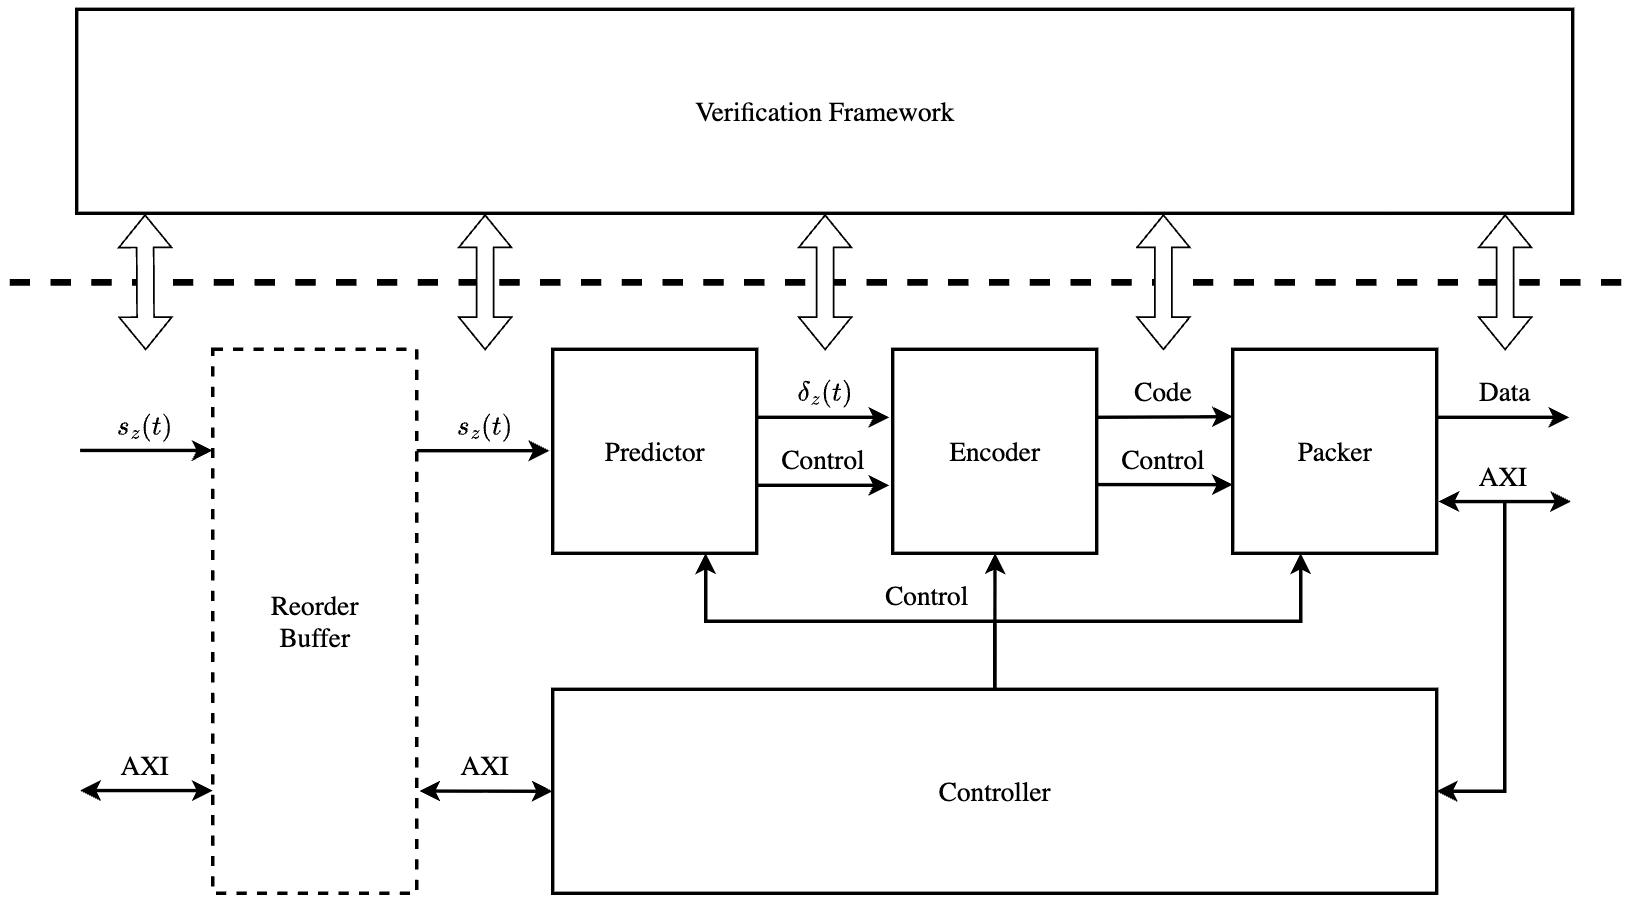
\includegraphics[width=1\textwidth]{figures/vorhaug-block.png}
	\end{center}
	\caption{Block diagram of \citeauthor{vorhaugHyperspectralImageCompression2024}. For easy integration into HYPSO, a reorder buffer reorders samples from \acrshort{BIP} to \acrshort{BIL}.}
	\label{fig:vorhaug-block}
\end{figure}

\begin{figure}[ht]
	\begin{center}
		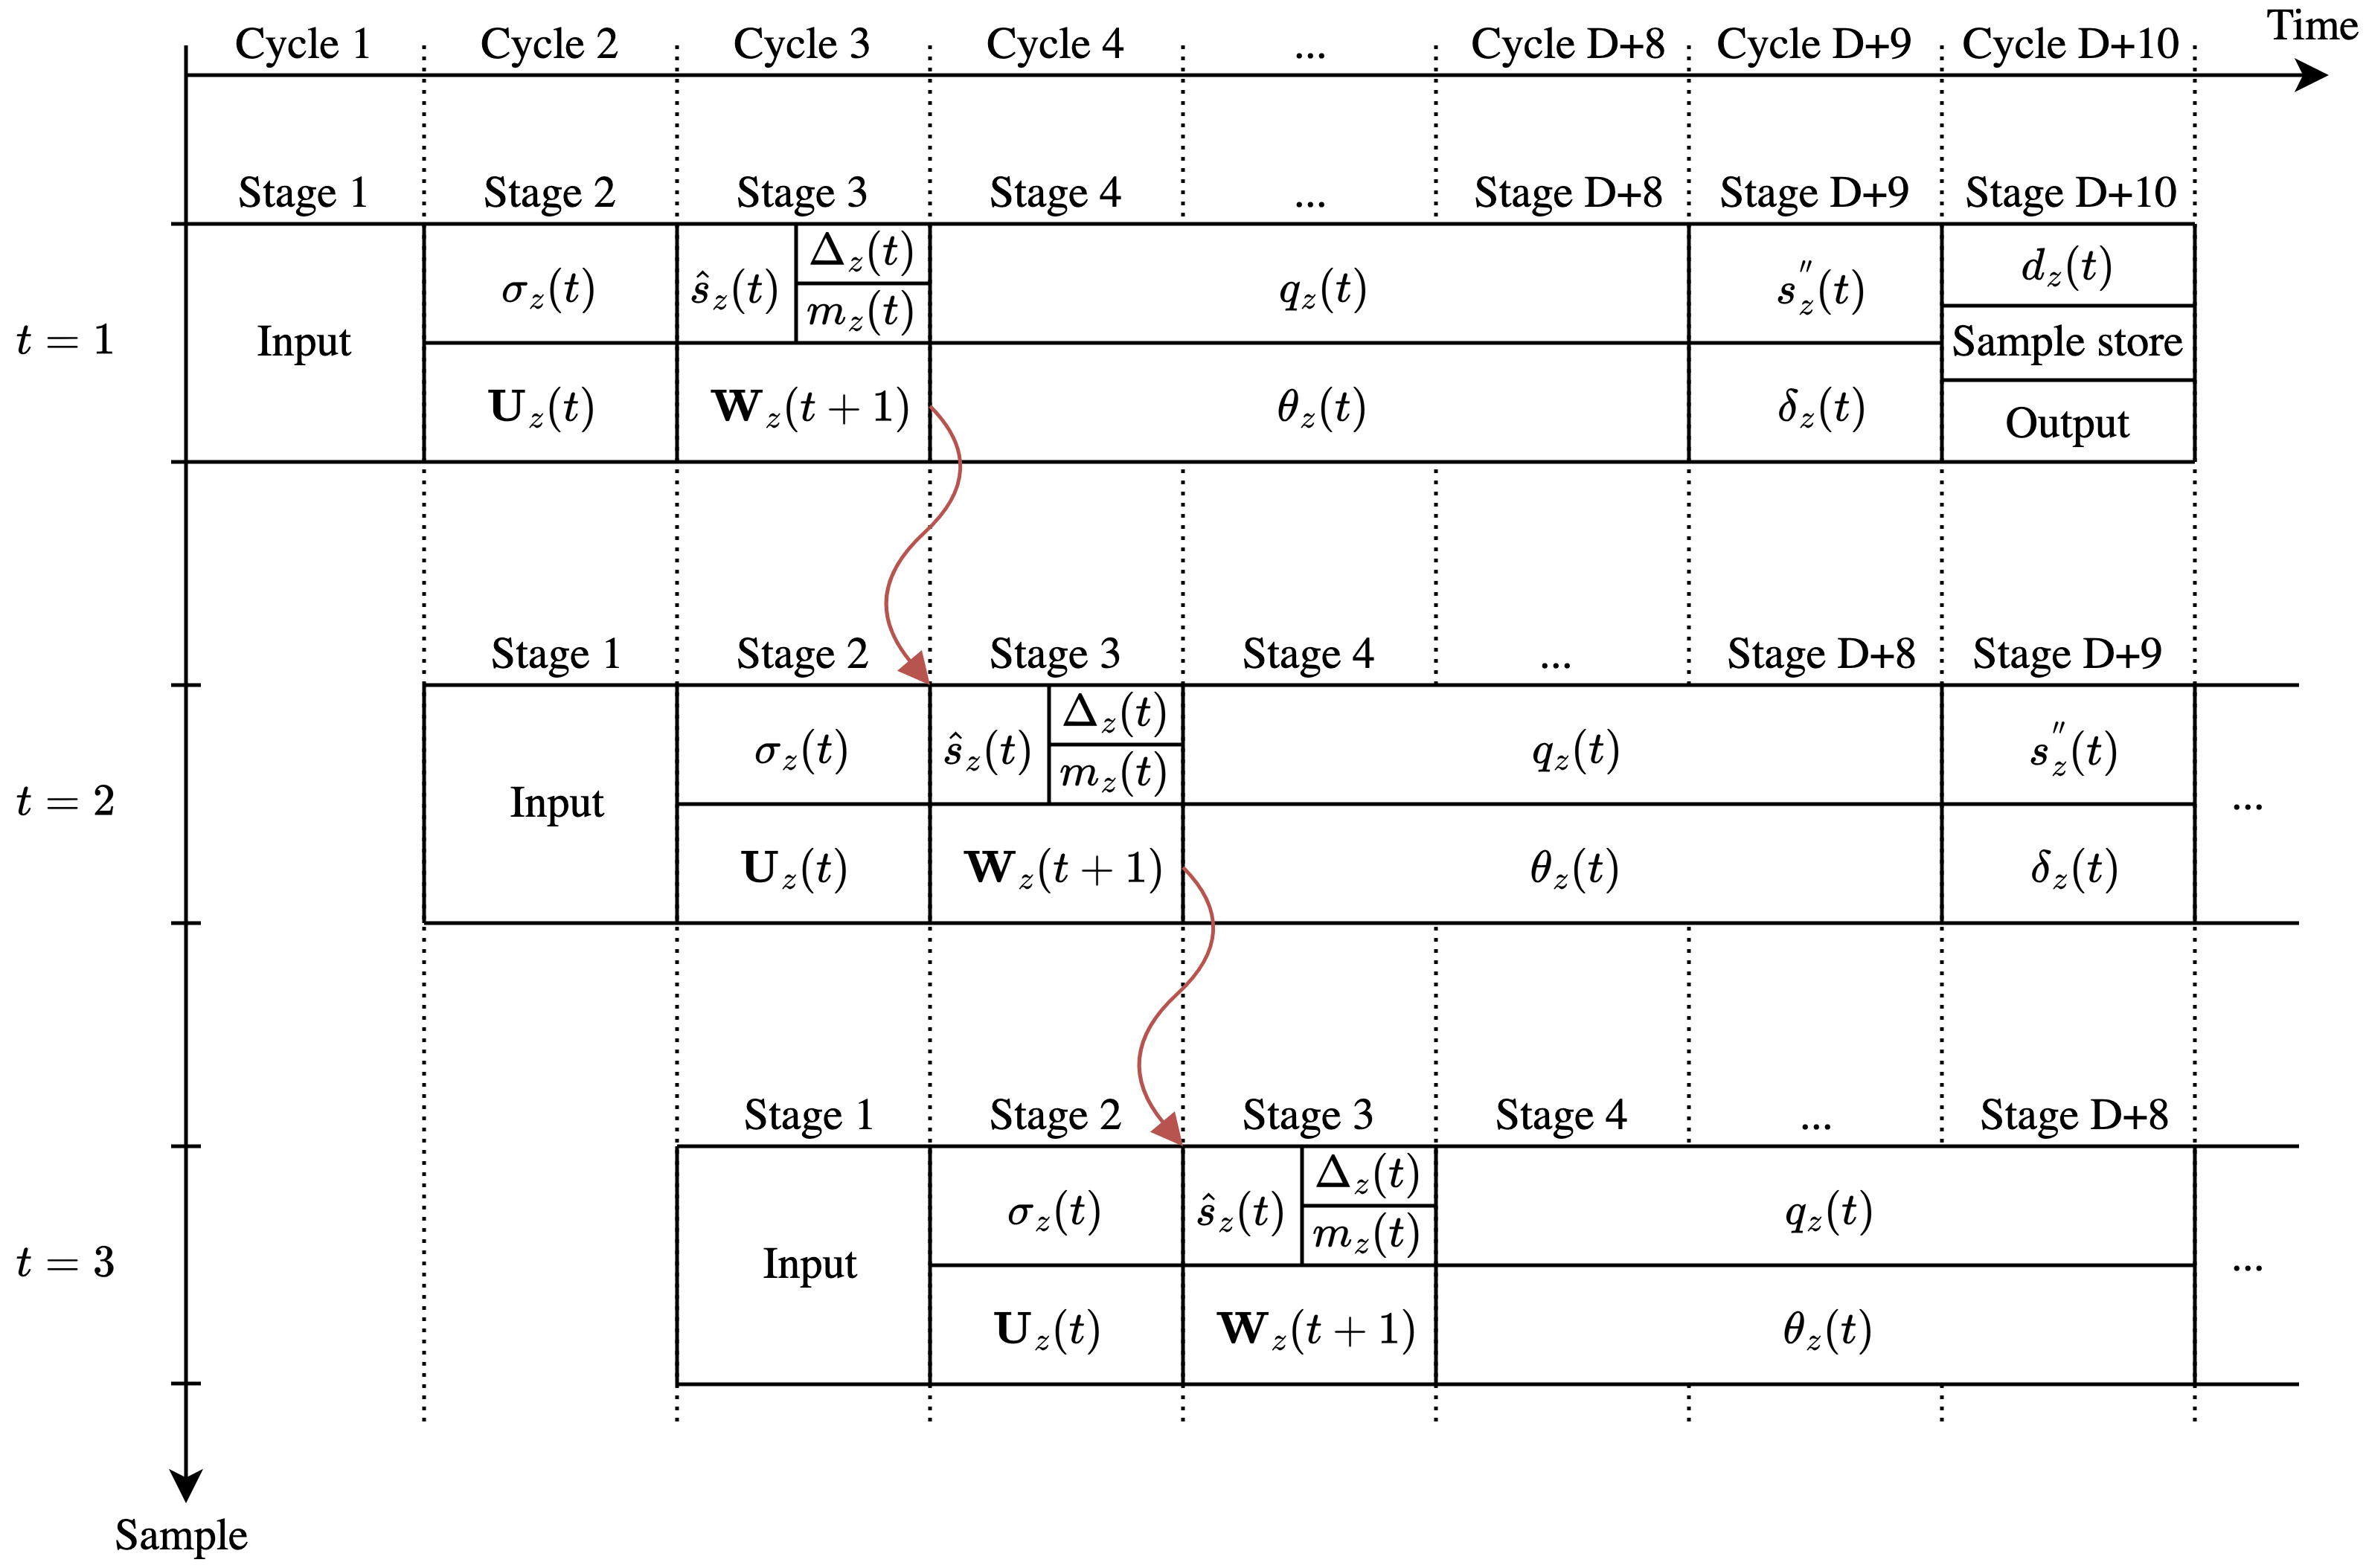
\includegraphics[width=1\textwidth]{figures/vorhaug-pipeline.png}
	\end{center}
	\caption{Full pipeline of \citeauthor{vorhaugHyperspectralImageCompression2024}. The indivisible weight update calculation in stage 3 restricts the throughput.}
	\label{fig:vorhaug-pipeline}
\end{figure}

\begin{figure}[ht]
	\begin{center}
		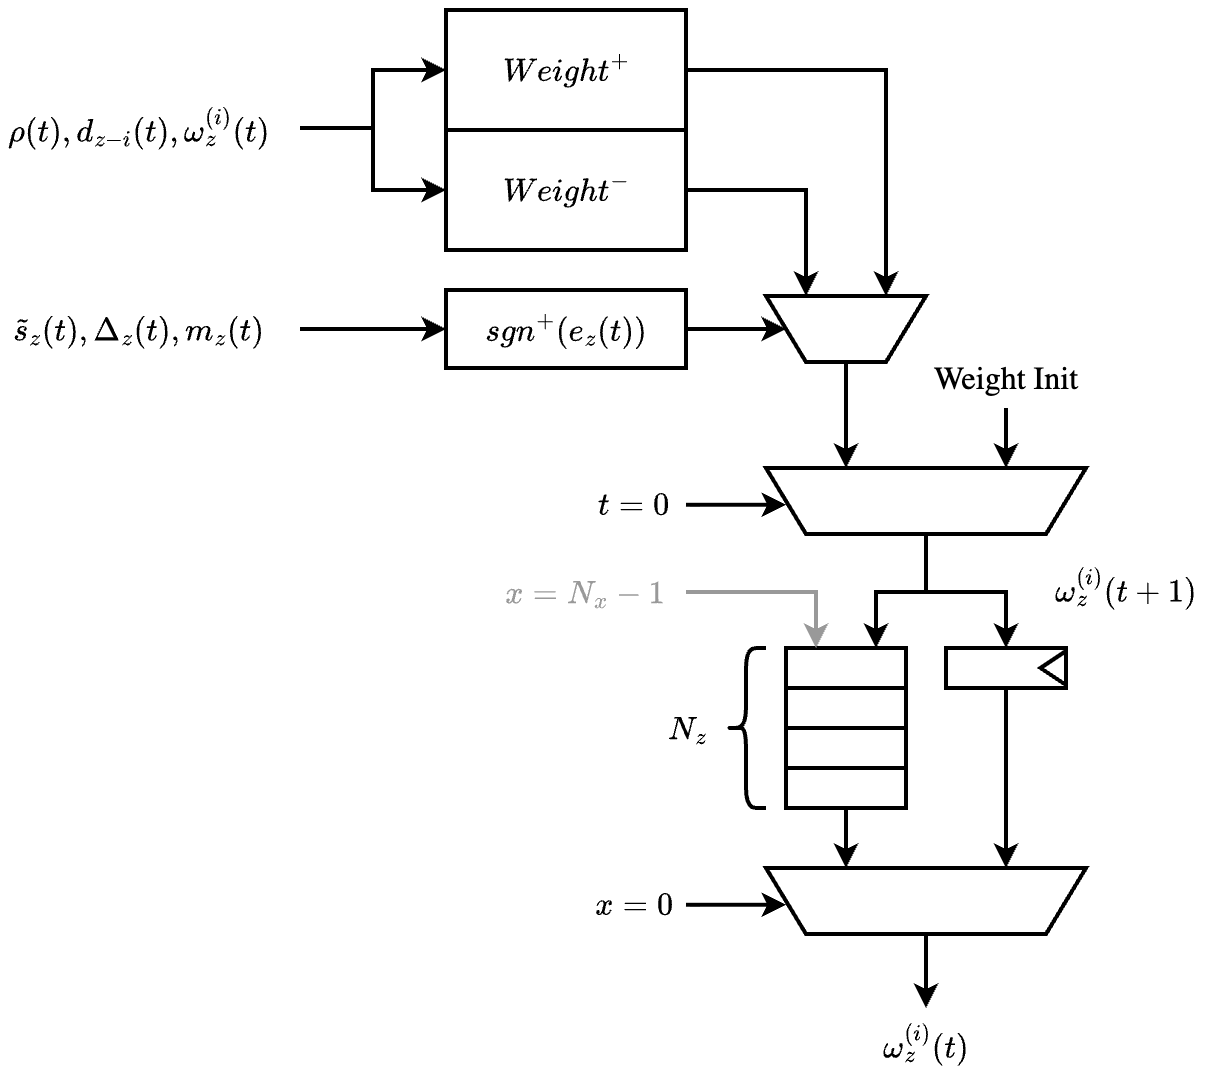
\includegraphics[width=0.8\textwidth]{figures/vorhaug-weights-hw.png}
	\end{center}
	\caption{Weight update stage of \citeauthor{vorhaugHyperspectralImageCompression2024} following the mathematical optimization approach proposed by \citeauthor{sanchezReducingDataDependencies2022}. Weight updates are calculated speculatively while the sign of the prediction error resolves.}
	\label{fig:vorhaug-weights-hw}
\end{figure}

\begin{figure}[ht]
	\begin{center}
		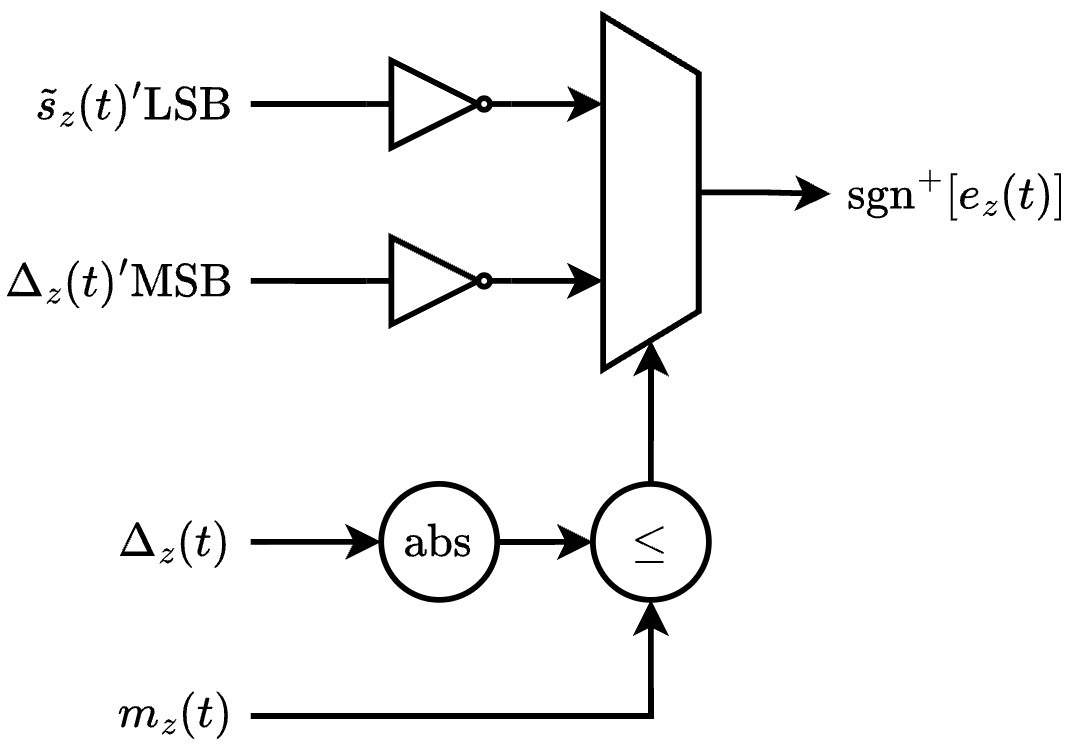
\includegraphics[width=0.5\textwidth]{figures/sign-block-diagram.png}
	\end{center}
	\caption{}
	\label{fig:sign-block-diagram}
\end{figure}

\begin{equation}
	\begin{cases}
		!\bigl(\tilde{s}_z(t)'{\mathrm{LSB}}\bigr), & \lvert \Delta_z(t) \rvert \le m_z(t), \\[6pt]
		!\bigl(\Delta_z(t)'{\mathrm{MSB}}\bigr),    & \text{otherwise}.
	\end{cases}
	\label{eq:sign-hw}
\end{equation}
